This chapter explains the Data Mining tasks that are introduced at Choicely through this thesis work. The first subchapter introduces setting in which this research is conducted. The reason behind this is to provide more insights over the introduction presented in Chapter \ref{section::introduction-to-the-choicely-voting-platform}. Secondly, learning about the system's core functionality related to this research provides a better understanding for the rest of this study. The second subchapter addresses this space and tells about the rules of contests and voting. The third subchapter introduces relevant insights on the company's data related to this research. This subchapter can provide interesting insights to all researchers, who conduct similar studies at companies or wishes to learn how data is typically stored in such research environment. Finally, the last subchapter argues for the relevance of the selected methods and explains how they are applied in this study. 

\subsection{Research setting}
    % why is the data analysis relevant from scientific research point of view?
    Performing scientific research on such data is interesting for multiple reasons. To begin with, at the time of this research Choicely did not utilize data analysis tools on the collected data. It is in the interest of the company and its customers to better understand what kind of audience was engaged in the past, what kind of content is more (or less) successful and what tendencies in user behavior can be extracted from the data. By doing so, both parties can provide better services and richer content to their targeted customers. Therefore, the introduction of data analysis and visualization tools at the company will greatly enhance business value of the firm, provide deeper understanding on the domain as well as the existing user base.   
    
    % how is Choicely different than other social networks or any other repository of user data?
    Secondly, Choicely can be looked at as a social network, because some of the pictures uploaded to the platform is generated by users. Users also have the possibility to express their appreciation or support towards some contest participants by spending votes on them. Similarly to social networking sites, where the "like" feature is often used \cite{jang2015noreciprocity, bakhshi2014faces} this phenomena can be looked at as a way of expressing personal opinion. 
    
    In comparison to most of the currently available social networks, voting platforms like Choicely are observed by the audience differently. On one hand, social media sites usually list posts or images on a feed, where there is theoretically no relation between the posts that follow eachother. % TODO citation
    On the other hand, contestants in the Choicely platform share similarities as they were nominated for the same contest. Accordingly, there must be some similarity among them as all are subjects of the contest's topic, rules and are competing for the best possible result. 

    % so what? Why is that important from user point of view
    This slight difference can make a big change in terms of user behavior. The focus moves from "what kind of content I like" to "which piece of content I like the most in comparison to the rest". Consequently, users will scan through some (or optimally all) of the contestants and make unconscious decisions upon whether to give vote(s) on certain contest participant(s). The users express their favor and support towards a subset of contenders, hence helping them to reach their ultimate goal: winning the contest. 
    % how can this contribute to user behavior and social media studies? 
    This uniqueness compared to other social networking sites offers a great possibility for research. Therefore, the hands-on goals towards the analysis are two-folded: 

    \begin{enumerate}
        \item identifying what kind of images among different contests users like, and
        \item what kind of content similar group of users like.
    \end{enumerate}

    % how computer vision is going to be utilized? 
    One of the challenges in connecting users with topics is that there is no indication on what the content on the participants' pictures is. Contest authors only assign categories to the contests to be created, which does not necessarily describe the entrants. Other researches have successfully utilized computer vision to gather meta data for the uploaded content in image sharing communities \cite{bakhshi2014faces, hu2014we}. 
    
    % what is the solution to this problem?
    Deriving from the success in previous studies \cite{hu2014we, farseev2015harvestingmultiplesources, han2016teensarefrommars, bakhshi2014faces}, computer vision is applied in this research to identify labels that appear on the participants' images. For instance, a beauty pageant's entry image may be labeled with meta data, such as "Beauty", "Photo Shoot", "Smile" and "Blonde". Similarly, a design contest entry might have topic labels, such as "Landmark" or "Architecture". Figure \ref{google_vision_labels} displays an example, where the Google Vision API was used to extract labels from images which were used in contests of Choicely.

    \begin{figure}[h] 
		\begin{center}
            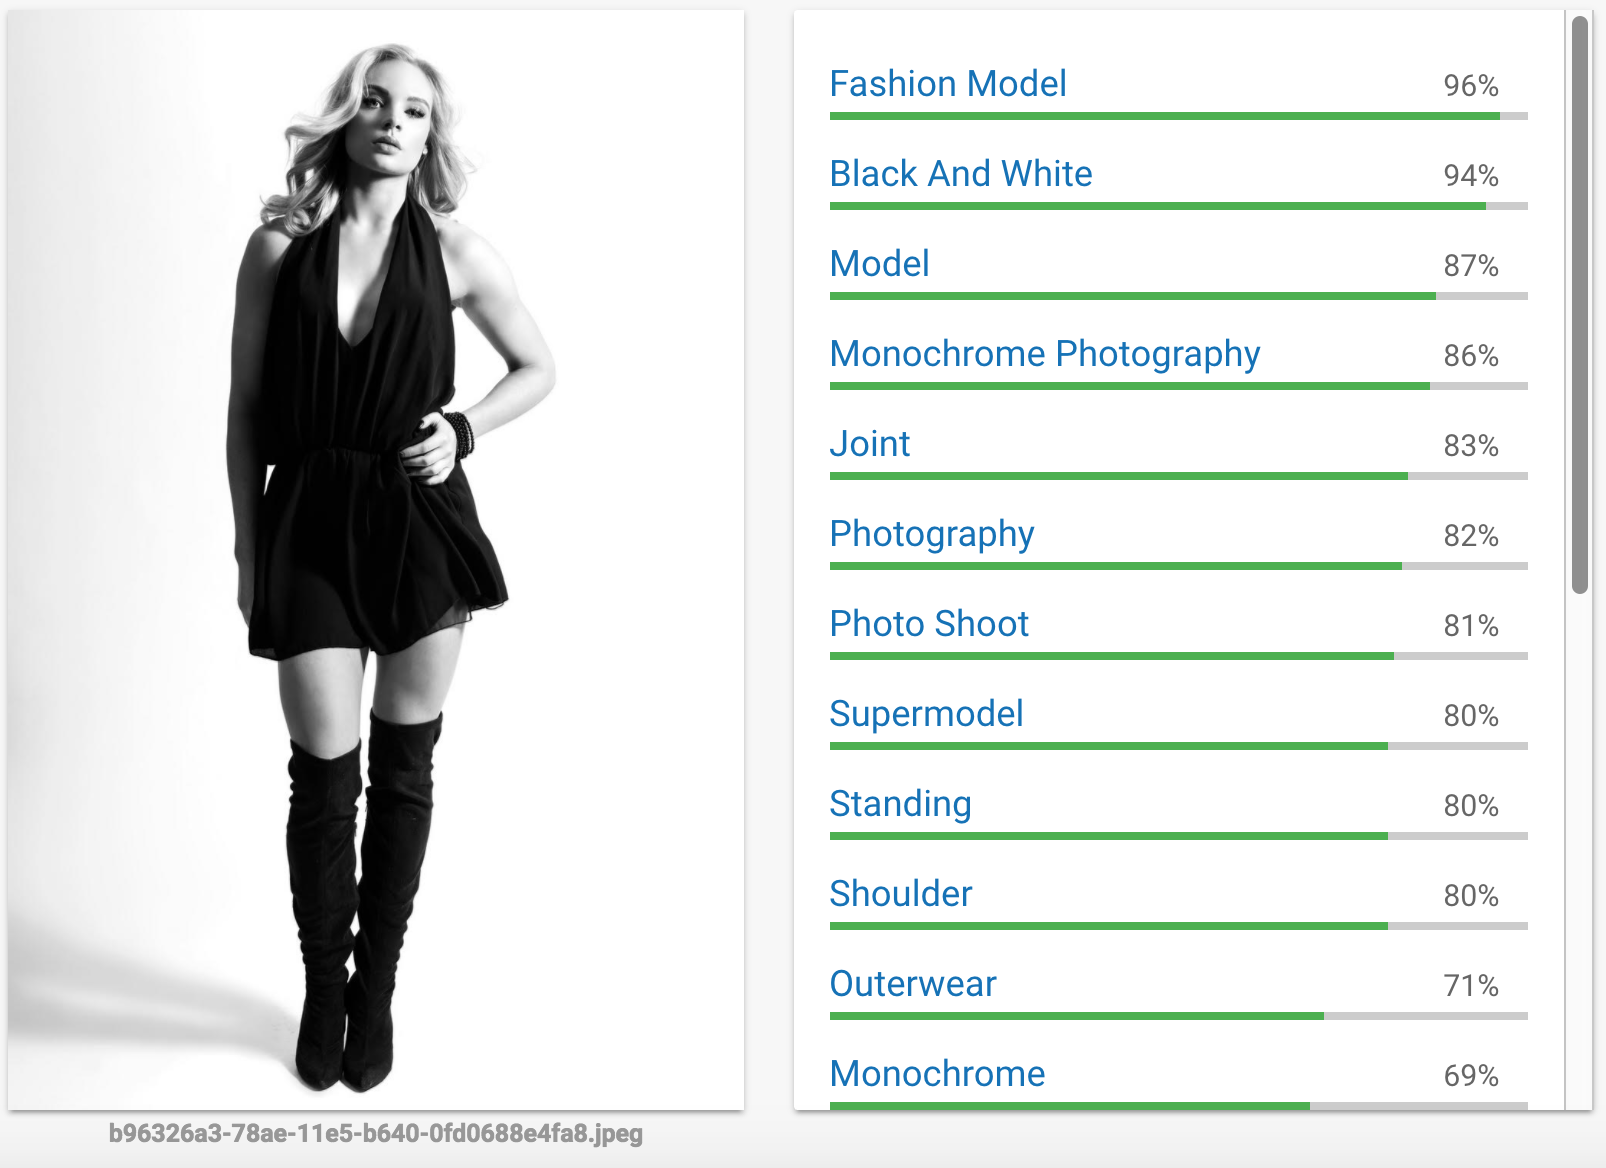
\includegraphics[width=0.8\textwidth]{images/google_vision_labels.png}
            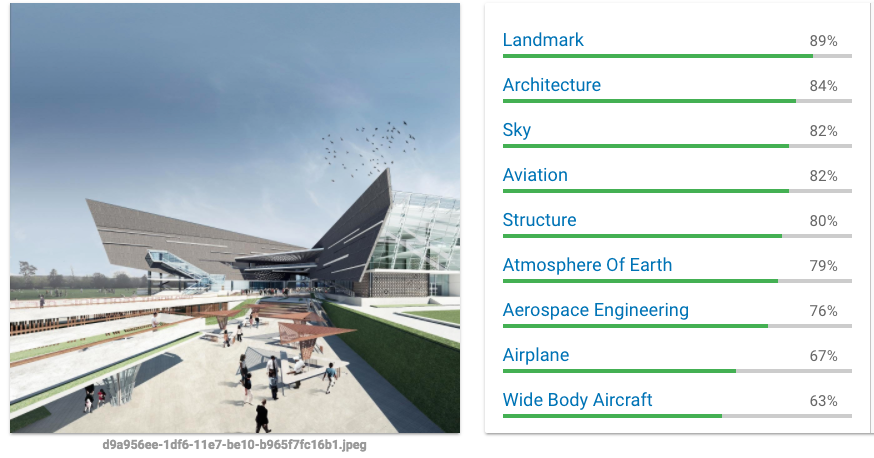
\includegraphics[width=0.8\textwidth]{images/google_vision_labels2.png}
			\caption{The labels identified by the Google Vision API on two of the contest participant's images.}
			\label{google_vision_labels}
		\end{center}
    \end{figure}

    % how are the labels used - what is the method performed on them? 
    Combining the identified labels and the vote data can provide information on user behavior. For instance it can be identified which demographic group of users like what kind of content, or the behavioral differences between two or more groups can be compared to eachother. Furthermore, this kind of information could be used to recommend new content in the platform to users which they have not seen before. Last but not least, it could be identified that which traits of participants contribute to more votes and engagement by users or certain user groups.  

\subsection{The voting mechanism and the user profiles}
% voting options
Various voting options are available for Choicely contests. The author of the contest has the choice of setting a limit on how many votes users can spend on individual participants or the whole contest in overall. For instance, if the maximum votes in the contest is set to 1, users can give exactly a single vote on one and only one participant. Configuration settings allow infinite votes as well. In this case, users may vote on all of the participants as many times as they like. Removing votes is possible, if the author has decided to enable this possibility. Votes cannot be modified after the contest has ended. Each contest has its own voting configuration. 
    
% free-silver-gold votes
On top of the regular free votes, contest authors may allow users to earn more votes (called "silver votes") by sharing the contest on social media or by watching adverts. Furthermore, contest authors can allow users to purchase more votes (called "star votes" or "gold votes") with exactly the same restriction settings as explained above. Note, however that the configuration for the three vote types are distinct for every contest. This means that the limitation on free/silver/star votes may differ for individual participants as well as the whole contest. For instance, a contest author may allow users to spend only 5 votes for free, but unlimited number of silver and gold votes in a contest. 

In this research, there are no distinctions made between the different vote types. That is, free, silver and star votes are considered as equal. The rest of this study makes no difference between the different vote types, but simply considers them as votes on contest participants, which is a sign of favor shown by the user towards the contest participants. Nevertheless, it would be interesting to separately study if there is any significant difference in how users spend different types of votes. 

Each user profile contains the features listed in Table \ref{user_profile_fields}. For the purposes of this research, the fields written in italic text in the table below are considered interesting part of user profiles. The three highlighted attributes are all categorical variables, that contain demographic information about users. By filtering the data using these demographic attributes, one can obtain data generated by targeted segments of users and compare those datasets. This way the behavior of the demographic groups can be studied, which provides answer to RQ3. To keep the scope of this research compact, only the country information of the users' location is utilized in this study (the state and city are not used).

\begin{table}[H]
    \centering
    \begin{adjustbox}{width=0.8\textwidth}
        \begin{tabular}{l|l}
            \textbf{Field}              & \textbf{Type} \\
            \hline
            Full name                   & Free text \\
            Profile picture             & Image \\ 
            Cover image                 & Image \\
            \textbf{\textit{Gender}}    & Male/Female/Other/Not chosen \\
            \textbf{\textit{Location}}  & Country, state and city \\
            Birthday                    & Datetime \\ 
            \textbf{\textit{Age group}} & 0-17/18-24/25-34/35-44/45-54/55-64/65+/Unknown \\
            Introduction/Bio            & Free text
        \end{tabular}
    \end{adjustbox}
    \caption{The list of fields and their types for each user profile.}
    \label{user_profile_fields}
\end{table}  

The demographic data is filled by the users at the time of signing up for the service. Contests require users to have a user profile in the Choicely platform. Choicely offers authentication through social media (Facebook and Google+) as a convenient option for users to sign up with one click. In this case, the social media platform provides information about the user's profile to Choicely, which allows the automatic population of the demographic data of the user. Optionally, user profiles in Choicely can be created through a regular sign-up process, where users pick a user name as their identities. In such case, their demographic data is unknown by default and it is up to the users to complete their profiles. 

% what kind of data is generated?
In sum, the user data in Choicely consists of the user profiles, which contain demographic information about the users, namely age group, gender and location. On top of that, contests have a number of participants with arbitrary number of votes that the users have already casted. The latter kind of data can be seen as digital footprints generated by users in the Choicely platform. The combination of these datasets sums up to the user data as introduced in the previous chapter and Figure \ref{user_data_venn} in this particular case. This is further supported with the meta data of contests and contest participants, which was explained in the previous subchapter.
    
\subsection{Data structure and retrieval}
    % architectural overview
    In order to better understand the data, the data structure and architecture of the Choicely platform is explained briefly in this subchapter. Most of the platform's data is stored currently in the Google Cloud Platform\footnote{\url{https://cloud.google.com}}, more specifically in Google Datastore\footnote{\url{https://cloud.google.com/datastore}} and Google BigQuery\footnote{\url{https://cloud.google.com/bigquery}}. Google Vision\footnote{\url{https://cloud.google.com/vision/}} is utilized as a computer vision service to gather the meta data for the contestants' images. 
    
    Google Datastore is highly scalable document database which is built on top of NoSQL technology \cite{google-datastore-overview}. By providing flexible storage, performant computing resources, encryption possibilities and high availability, the service can serve wide range of applications and various type of business data of companies \cite{google-datastore-overview}. Google BigQuery is a data warehouse for enterprise purposes, large-scale data storage, processing and analysis \cite{google-bigquery-overview}. Most of Choicely's data is stored in Google Datastore, however the computer-vision identified tags of the participants' images (Figure \ref{google_vision_labels}) are located in Google BigQuery at the present time.
    
    The data is structured into entities in both Datastore and BigQuery. There is parent-child connection between entities, which are key for the retrieval of some of the unique entities. For instance, contests belong to Users or Brands (as contest organizers), which are separate entities in the platform. Certain entities can be identified by multiple parent entities. Entities that have no parent(s) can be identified with their unique identifiers and indexed with some other fields. For example, users can be filtered by gender and age group, or unique identifier. 
    
    The data is generated by contest organizers, who create contests in the platform and users, who cast votes on their favorite participant(s) in the contests through one of the interfaces explained in Figure \ref{choicely_platforms}. The contest participants' images are identified automatically via the combination of Google Vision\footnote{\url{https://cloud.google.com/vision/}} and Google Cloud Functions\footnote{\url{https://cloud.google.com/functions/}} once they are uploaded to the database. Google Vision is another component of the Google Cloud, which provides powerful image analysis solutions for software developers \cite{google-vision-overview}. In this study, the usage of this component is limited to the classification of the content on the images as explained above. Google Cloud Functions are used to be able to automatically assign the labels to the images so that the manual work can be reduced to the least minimum. 

    Similarly to SQL join statements, the aforementioned identifiers and the parent-child relationship can be used to join list of various entities together. This property is used to aggregate and prepare data for the purposes of the analyses to be performed. Accordingly, the Contest, User, ContestVote, Vote and ImageLabel entities are joined together via their connections to construct the data structure displayed in Table \ref{association_analyisis_data}. This data structure establishes the basis of the Association Analysis, which is performed to address RQ3. 

    Figure \ref{choicely_architecture} displays the architecture of the Choicely platform on a high level. The Users of the system use the Choicely clients on their mobile or personal computer to create new contests or cast votes in the existing ones. 
    % From the point of view of this thesis work there are no significant differences between the two entitites, their role is simply to provide engaging content to a large number of users. Users then on the other hand participate in the contests by casting votes on the contest participants. 
    The Vote and Contest data is collected and stored to the databases that are hosted by Google Datastore. The data analysis is then performed by the Data Analysis framework, which is used by either a data analyst or an automatic service. This thesis work is devoted to establish the core functionality of this framework through this thesis work. Finally, Knowledge Discovery and Data Visualization is performed on the output of the framework. 

    \begin{figure}[h] 
		\begin{center}
            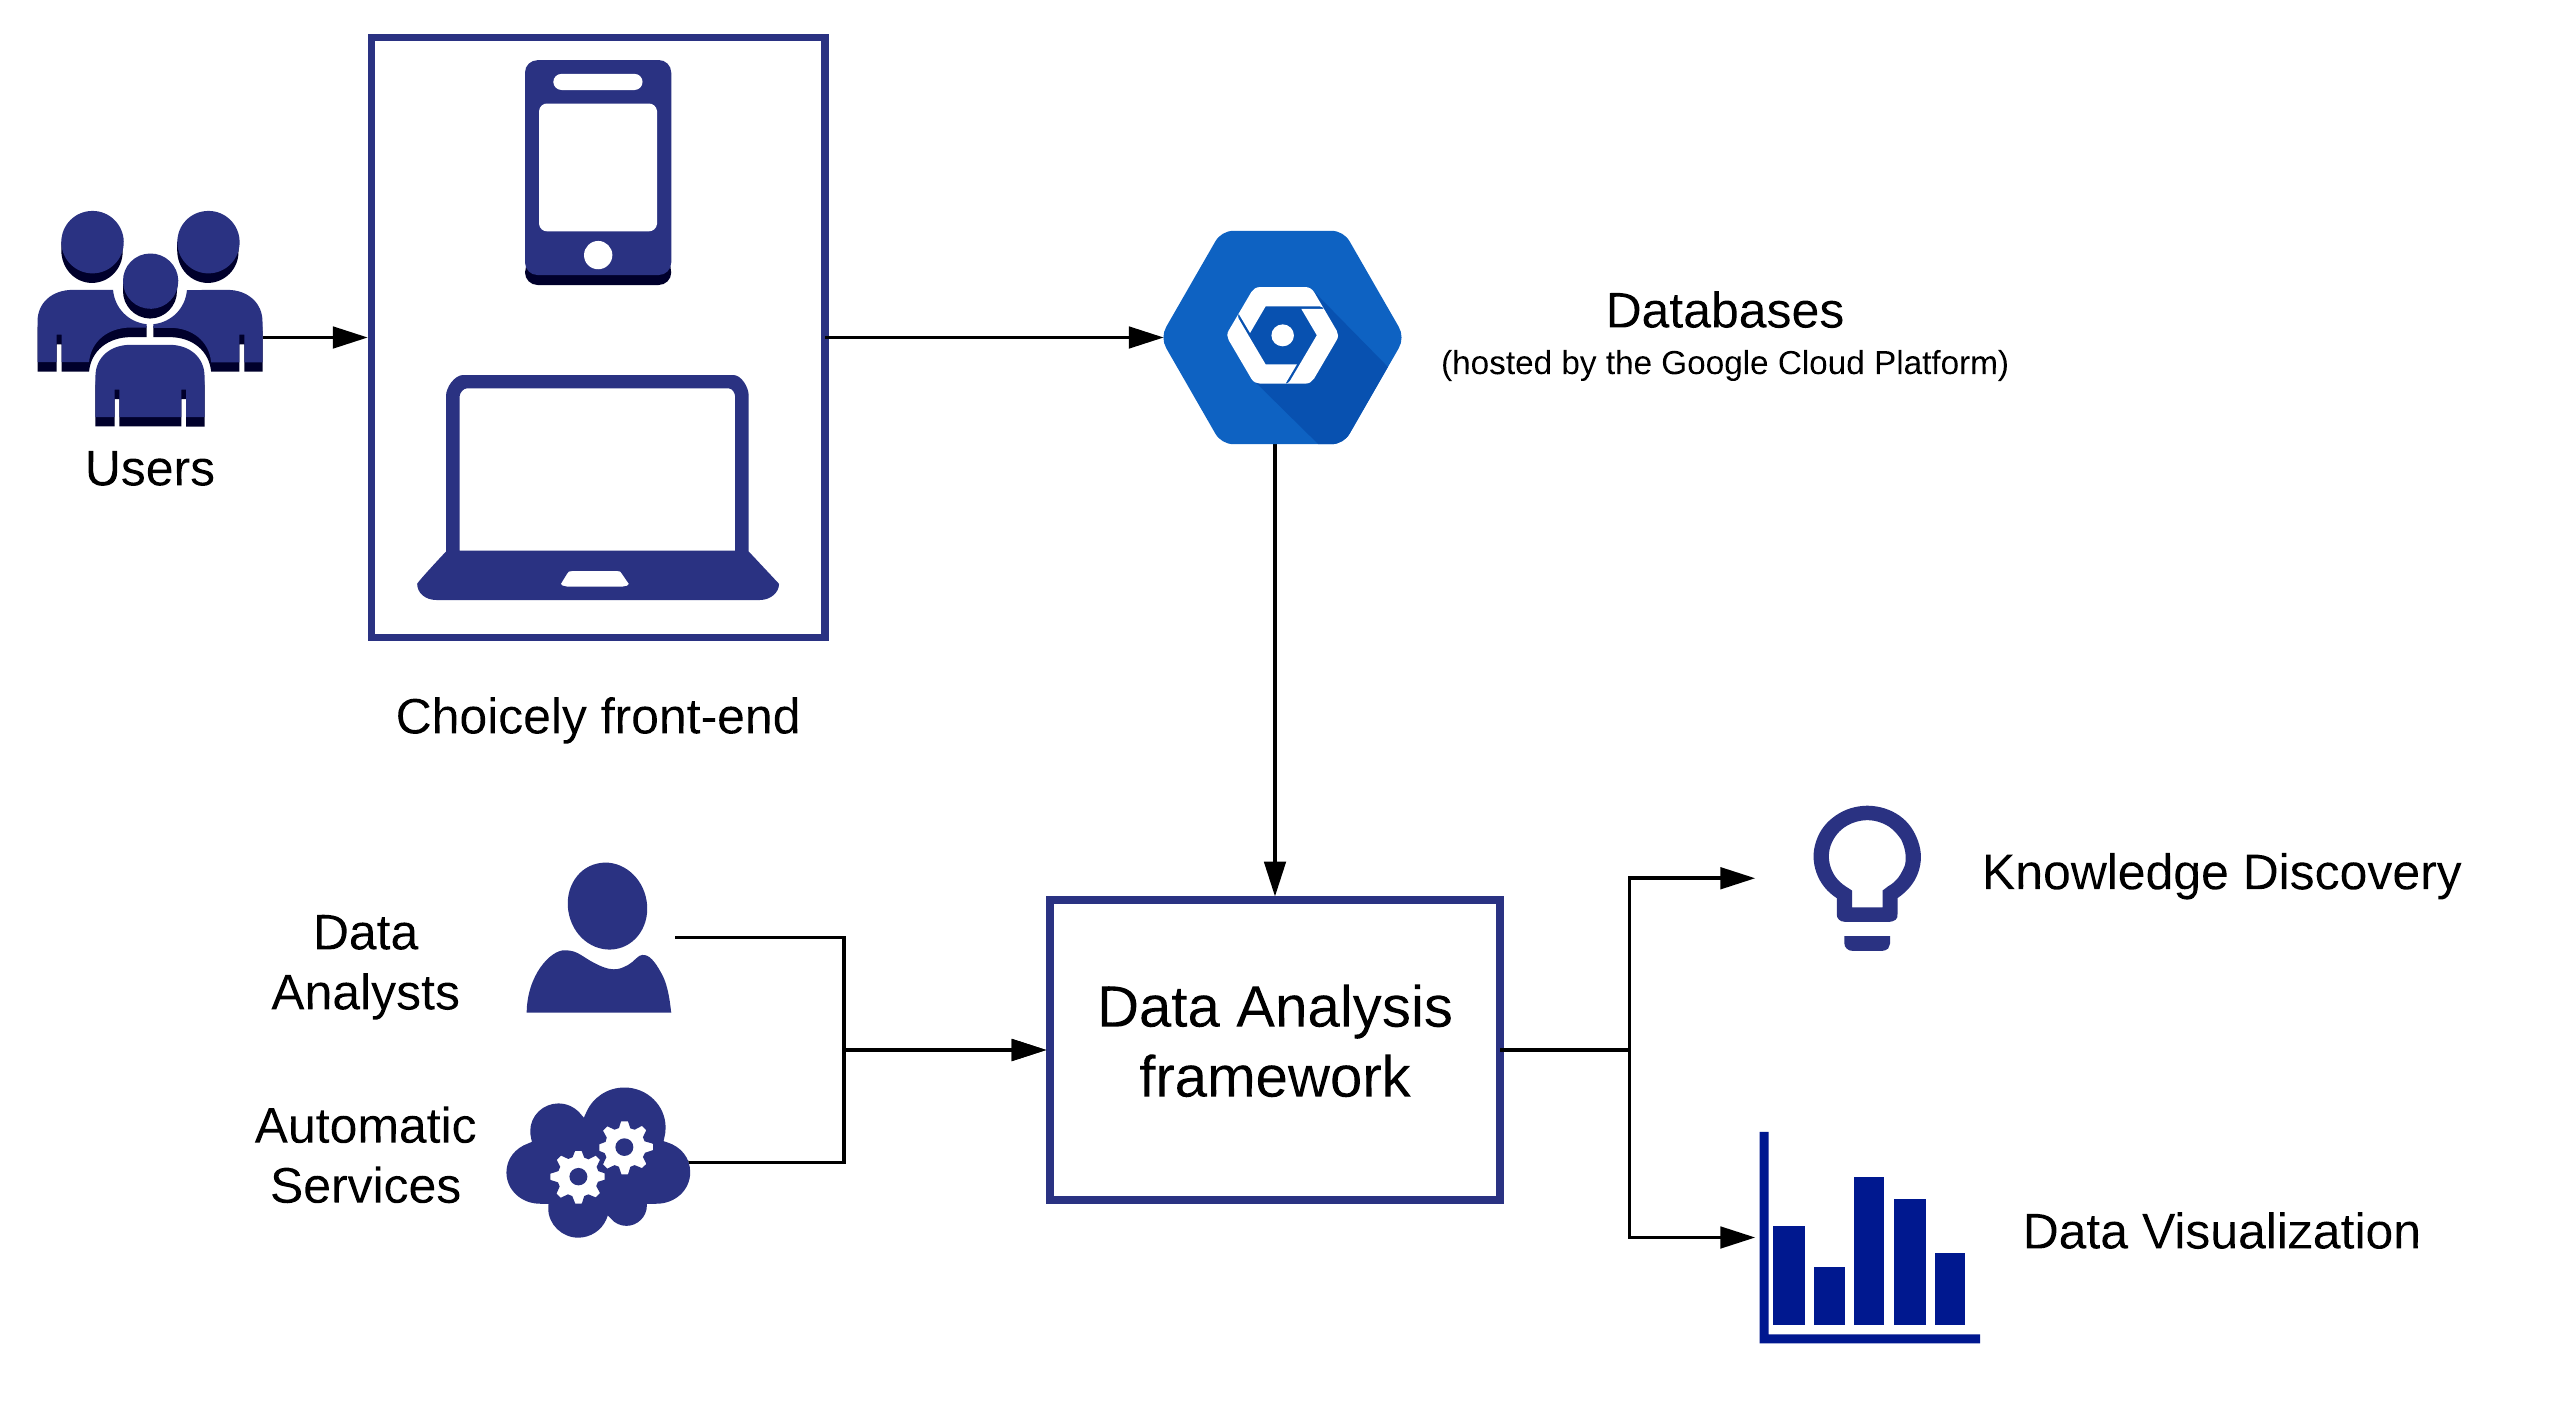
\includegraphics[width=0.8\textwidth]{Images/architecture.png}
			\caption{The brief architectural overview of the Choicely platform.}
			\label{choicely_architecture}
		\end{center}
    \end{figure}

    %\subsection{Knowledge Discovery and Data Visualization}
    \subsection{Applying the chosen methods}
    To answer RQ2 and RQ3 (presented in Chapter \ref{section::reseach_questions}), the chosen methods presented in Chapter \ref{section::methodology} are applied in relation to Choicely's data. The paragraphs to follow elaborate a more in depth, what kind of data is used in case of the Choicely to answer the stated questions. On top of that it is explained, how the data was transformed in order to achieve the results. Data records collected before $1^{st}$ January, 2018 are used for the analyses. 

    % what is the goal of EDA? How is it used in this research? 
    The EDA fundamentally focused on studying the user engagement in contests and over the contest categories. In other words, the EDA is performed on the data extracted from the Contest entities in Choicely. This choice is done with the aim of addressing the research space of RQ2.
    
    Contests have a few attributes which can help answering RQ2. To gain an understanding on how many users are typically engaged in contests, the number of unique voters is studied in comparison to the number of contests. The number of unique voters means the users, who have voted on at least one participant in a contest. This value can be retrieved for all contests in the platform. Contests can be filtered by their categories which is another approach towards finding answers to RQ2. Similarly to studying the number of unique voters over contests, the same metric is applied to all contest categories. By looking into how many users have voted in which kind of contests, one can get a grasp on the kind of contests that tend to attract more users.

    To answer RQ3, Association Analysis using the Apriori algorithm is performed. In order to be able to execute the analysis, some preprocessing has to be done. The list of labels extracted from the participants in the contest are listed for each transaction alongside with the voters' demographic data. In other words, the data has to be transformed such that the input contains rows of the voters' demographic attributes and the computer-vision identified labels from the participants' images. In order to achieve this, the User, Contest, ImageLabel and Vote tables are joined together. The retrieved data is combined as shown in Table \ref{association_analyisis_data}. One challenge in constructing this data was that these pieces are located in different storage places (Google Datastore and Google BigQuery), which often happens at companies in software development field. 

    \begin{table}[H]
        \centering
        \begin{adjustbox}{width=0.8\textwidth}
            \begin{tabular}{l|l|l|l}
                \textbf{Gender} & \textbf{Age group} & \textbf{Country} & \textbf{Labels} \\
                \hline
                female & 25-34 & fin & ['fashion model', 'hair', 'model', 'beauty', '...] \\
                male & 18-24 & fin & ['dark hair', 'hair', 'model', 'smile', '...] \\
                male & 65+ & fin & ['fashion model', 'hair', 'shoulder', 'beauty', '...] \\
                female & 18-24 & swe & ['fashion model', 'hair', 'model', 'beauty', ...] \\
                male & 18-24 & hun & ['beauty', 'blond', 'human hair color', 'model', ...]
            \end{tabular}
        \end{adjustbox}
        \caption{The format of the data used for Association Analysis (the records dispalyed in the table are only examples).}
        \label{association_analyisis_data}
    \end{table}

    After transforming the data, the Apriori algorithm is applied to calculate the itemset supports. This can be done on arbitrary amount of vote transactions as long as they have been transformed to the desired format. However, there are certain cases when it makes sense to perform the analysis. For instance, the analysis can be performed 

    \begin{enumerate}
        \item on transactions of a single contest: this way contest organizers get a chance to analyze their engaged audience and seek the tendencies in their behavior,
        \item on transactions extracted from the complete dataset: this way one can attempt to find patterns in how users behave on the system-level,
        \item on transactions of a targeted group of users: this approach allows to understand the preferences of a desired group of people across multiple contests,
        \item on transactions of a single user: this way the behavioral patterns of the individual user can be studied and analyzed. 
    \end{enumerate}

    It would be interesting to take a look into all of these aspects, however the scope of this thesis work limits the analysis to be performed. On top of that, items 3 and 4 might go into "too personal" directions, hence interfere with privacy issues and raise ethical concerns. In order to keep the scope of the analysis on a reasonable level, items 1 and 2 in the above list are taken in the analysis and the rest are discarded. 
    
    Using the approach explained above, the support of the itemsets extracted from the labels can be calculated. The support in this case tells the percentage of votes, which were casted on an itemset of discussion. For instance, \emph{S(\{"beauty", "blonde"\}) = 0.6} would mean that 60 \% of all votes were casted on participants whose images contained the \emph{\{"beauty", "blonde"\}} itemset. Likewise, if the list of vote transactions is filtered by one of the demographic attributes, the same can be said for the investigated group of users. The itemsets in this analysis are all extracted by first stating conditions for the value of the demographic group (i.e. gender is male), which puts a condition next to the value. Note that many researches in the field of Data Mining use the term confidence for such conditional associations. In this reserach, the term support is used for this purpose and context consistently.

    To ensure that the algorithm's runtime is not too long, the \emph{minsup} value is set to 0.05, which corresponds to 5 \% support. This means that all itemsets, that have less support than this value for all demographic groups, are pruned during the progression. On top of reducing runtime, this threshold is set to eliminate less interesting itemsets and keep only the interesting ones on the output.

    The result of the Apriori algorithm then can be collected into a table displayed on Table \ref{itemset_supports_format}. This table shows the itemsets as rows and the targeted group of users as columns. The values in each columns correspond to the support values of the itemsets for the given group of users in the set of transactions that was fed into the algorithm. 

    % TODO consider if the next paragraph is needed at all
    % Note that despite the values in the rows are probabilities, their values do not have to sum up to $1.0$. This is because each value in the table tells the probability, that a randomly selected transaction will contain the itemset (row), given that the vote was casted by a person who belongs to the target group (column). In other words, the probabilities of the itemsets for the demographic groups are independent from eachother.

    \begin{table}[H]
        \centering
        \begin{adjustbox}{width=1\textwidth}
            \begin{tabular}{l|c|c|c|c}
                X & \emph{S(X|gender=male)} & \emph{S(X|gender=female)} & \emph{S(X|gender=other)} & \emph{S(X|gender=not\_specified)} \\
                \hline
                \emph{\{"beauty", "blonde"\}} & 0.6 & 0.8 & 0.15 & 0.25 \\
                \emph{\{"cat", "fluffy", "cute" \}} & 0.6 & 0.1 & 0.5 & 0.0 \\
                \emph{\{"sea", "photo shoot", "model"\}} & 0.0 & 1.0 & 0.33 & 0.65 \\
                \emph{\{"building", "architecture"\}} & 1.0 & 0.0 & 0.25 & 0.0 \\
                \emph{\{"building"\}} & 1.0 & 0.0 & 0.33 & 0.0
            \end{tabular}
        \end{adjustbox}
        \caption{The output format of the Association Analysis comparing genders, where X is the itemset and S is the support (the records dispalyed in the table are only examples).}
        \label{itemset_supports_format}
    \end{table}

    On top of the support values, lift is calculated and studied for the extracted itemsets. The goal of these calculations are to study attraction towards itemsets in relation to their presence in the contest. Despite the fact that lift is based on the support values, it helps studying not only the frequent itemsets, but also the improvement gained by the associations. This helps to compare differences between demographic groups and to better understand the attractiveness of itemsets.

    The lift values can be collected into a table displayed on Table \ref{itemset_lift_format}. Similarly as the itemset supports were gathered, this table shows the itemsets as rows and the targeted group of users as columns. The values in each columns correspond to the lift values of the itemsets for the given group of users in the set of transactions that was fed into the algorithm. 

    \begin{table}[H]
        \centering
        \begin{adjustbox}{width=1\textwidth}
            \begin{tabular}{l|c|c|c|c}
                X & \emph{L(X|gender=male)} & \emph{L(X|gender=female)} & \emph{L(X|gender=other)} & \emph{L(X|gender=not\_specified)} \\
                \hline
                \emph{\{"beauty", "blonde"\}} & 2.0 & 2.5 & 0.25 & 0.33 \\
                \emph{\{"cat", "fluffy", "cute" \}} & 1.25 & 0.05 & 1.0 & 0.0 \\
                \emph{\{"sea", "photo shoot", "model"\}} & 0.0 & 3.0 & 1.0 & 2.0 \\
                \emph{\{"building", "architecture"\}} & 4.0 & 0.0 & 1.0 & 0.0 \\
                \emph{\{"building"\}} & 3.0 & 0.0 & 1.0 & 0.0
            \end{tabular}
        \end{adjustbox}
        \caption{The output format of the Association Analysis comparing genders, where X is the itemset and L is the lift (the records dispalyed in the table are only examples).}
        \label{itemset_lift_format}
    \end{table}

    In this imaginary example, the lift value \emph{L(\{"building"\}|gender=male) = 2.0} suggests, that the support for "building" among male voters is two times as probable than "building" appearing on a randomly chosen contestant's image from the studied dataset. If the lift value is 1.0, then the probabilty of finding the itemset in the targeted group's vote transactions is the same as on the images in the contest. In other words this means, that the group shows no more and no less attraction towards this content than what is already available in the data. This case may occur for instance, when the same label appears on every image in the contest (its support is 1.0 for all transactions). Hence, this case is not considered interesting. Finally, lift value less than 1.0 suggests less attraction for the itemset, which can also suggest interesting findings.

    In order to better understand the results of the Association Analysis, first a single contest (Miss Suomi 2017\footnote{\url{https://choicely.com/contest/164f52c7-9df8-11e7-b3c9-d1a0f88250ad}}) is looked at more carefully. By looking at a single case study, the results can be analyzed and interpreted in a smaller scope and hence be understood easier. Secondly, the results of the analysis performed on the system-level are presented and interpreted briefly. This approach is chosen to demonstrate the capabilities and the potential of the technique in both smaller and larger datasets.

    The Miss Suomi 2017 contest has been hosted in the Choicely platform late September, 2017. The data used for the analysis in this contest consists of 176 votes from 73 users in overall. There are 10 participants in the contest, who were photographed while dressed in white cocktail dresses on a shore of a lake or sea. Each photo has one and only one participant. Each participant has only one and only one photo in this contest. 
    
    Depending on how many individual participants the chosen transactions target, the number of itemsets (hence the number of rows) grows rapidly. Also the number of demographic groups (hence the number of columns) may differ depending on which the property is used from the users' profile. Essentially, the number of categorical groups for genders can go up to 4, for age groups up to 7 (see Table \ref{user_profile_fields}), but many more for location-based groups. As a conclusion it can be said that despite the supports are obtained, most likely their number will be too overwhelming to look at and analyze. Furthermore, one might assume that there patterns and structural trends in the support values, for instance some itemsets may share similarities, while others may differ from eachother in terms of their support values.

    % Finally, Co-Clustering is utilized on the calculated supports 
    For this reason, the Co-Clustering method is used to identify if any itemsets or demographic groups show similarities in the voting data. The method is applied on the output of the Association Analysis displayed in Table \ref{itemset_supports_format}. More precisely, only the matrix of support values is taken as the input of the Co-Clustering method, which is an matrix of real values on the range of \emph{[0.0, 1.0]}. 
    
    A simplified example output of the method is displayed in Table \ref{coclustering_output_format}. As shown, the support values in the cells with the same background color show similarities in their values. For instance, the support values in the green cluster are all 1.0, while the red cluster contains values that are also somewhat similar. This suggests that these itemsets and demographic groups are similar in nature. It can be seen, that this representation adds a layer on top of the output of the previous Association Analysis step (Table \ref{itemset_supports_format}) by reorganzing and clustering the rows and columns of the data matrix. By applying Co-Clustering, the closely-related itemsets and the groups are clustered together and grouped closeby, which facilitates the interpretation of the results. 

    \begin{table}[H]
        \centering
        \begin{adjustbox}{width=1\textwidth}
            \begin{tabular}{l|c|c|c|c}
                X & \emph{S(X|gender=male)} & \emph{S(X|gender=female)} & \emph{S(X|gender=other)} & \emph{S(X|gender=not\_specified)} \\
                \hline
                \emph{\{"beauty", "blonde"\}} & \cellcolor{blue!25}1.0 &  0.00 &  0.05 &  0.0 \\
                \emph{\{"cat", "fluffy", "cute" \}} &  0.0 & \cellcolor{red!25}0.75 & \cellcolor{red!25}0.70 &  0.0 \\
                \emph{\{"sea", "photo shoot", "model"\}} &  0.0 & \cellcolor{red!25}0.66 & \cellcolor{red!25}0.90 & \cellcolor{green!25}1.0 \\
                \emph{\{"building", "architecture"\}} &  0.0 &  0.00 &  0.10 & \cellcolor{green!25}1.0 \\
                \emph{\{"building"\}} &  0.5 &  0.00 &  0.00 & \cellcolor{green!25}1.0
            \end{tabular}
        \end{adjustbox}
        \caption{An example output of the Co-Clustering algorithm itemset supports by comparing genders for \emph{k = 3} clusters. X is the itemset and S is the support. The clusters are highlighted with different colors (the records dispalyed in the table are only examples).}
        \label{coclustering_output_format}
    \end{table}
    
    The implementation is done with the help of the bicluster module \cite{scikit-bicluster} of the popular scikit learn package \cite{scikit-learn}. The Spectral Co-Clustering class is used for the analysis, which proposes to pinpoint biclusters with higher values than others according to the documentation \cite{scikit-bicluster}. The algorithm treats the input matrix as a bipartite graph, in which the rows and columns are nodes and the values in the cells are the weighted edges between them \cite{scikit-bicluster}. This logic suits the input matrix, as the higher support values in the cells represent stronger attraction between the itemsets and the demographic groups.

    It is important to highlight in advance, that the chosen algorithm assigns one column and row exactly to a single cluster. As a result, the yielding clusters do not overlap and cells can not belong to more clusters. The reason behind choosing this particular algorithm lies in its simplicity and the applicability to the problem. This can be seen as a limitation to this particular algoritm, nevertheless the potential viability in this setting of the approach can be discovered and analyzed. 

    Using this approach, the clusters that are similar are going to be organized close to eachother. The algorithm's input requires a \emph{k} value, which corresponds to the number of clusters to seek. The cluster labels are attached to each row and column respectively, which suggests the itemsets and demographic groups that belong to the same cluster. In the performed analyses, the k value of the Co-Clustering algorithm is set to $4$.  

    By knowing the clusters, one can conclude if there are tendencies among demographic groups in terms of behavior. For instance, if the age group 65+ and 0-17 would be assigned in the same cluster by the algorithm, that would prove the similar behavior of the users in these two groups. In other words this would mean, that the certain kind of content leads to the engagement of both of these groups, but not necessarily the others. This can be valuable information to marketing professionals in the situation, when they wish to target a specific group of discussion. The demographic traits could be further combined in theory (e.g. male teenager users from Finland), however this deep analysis is out of the scope of this thesis work. 